\subsection{Design}\label{Design}
These components form the core functionality of FDMremote, and is used to defined a \texttt{Network} object.

\subsubsection{CreateNetwork (Create)}\label{Create}
This component generates a Network object.
\begin{figure*}[h]
    \centering
    
\includegraphics[width = 3cm]{Figures/Create}
\end{figure*}
Inputs:
\begin{itemize}
    \setlength\itemsep{0.05em}
    \item \textbf{Curves} (C): list of curves that define the edges of the network. Only the start and end points are considered: curved lines will be converted into straight edges.
    \item \textbf{Anchors} (A): list of points that define the fixed nodes of the network. A minimum of 3 is required.
    \item \textbf{Force Density} (q): either a single value $[force/length]$ to apply to all edges or a list of values (of equal length to C) for individual force densities. {\color{gray} Default: 1.0}
    \item \textbf{Tolerance} (tol): snapping tolerance when calculating topology of network. This is the search sphere radius at the ends of each edge to determine which edges have shared nodes, and which nodes are defined as anchors. {\color{gray} Default: 0.1}
\end{itemize}

Output: a \textbf{Network} object.

\subsubsection{QByLayer (LayerQ)}\label{LayerQ}
Assign specific force densities for edges in specific layers.

\begin{figure*}[h]
    \centering
    
\includegraphics[width = 3cm]{Figures/Qbylayer}
\end{figure*}

Inputs:
\begin{itemize}
    \setlength\itemsep{0.05em}
    \item \textbf{EdgeGUIDs} (GUIDs): GUIDs of all input network edges.
    \item \textbf{LayerNames} (Layers): Names of layer(s) of edge groups. {\color{gray} Default: "Default"}
    \item \textbf{ForceDensities} (Q): Force density to assign to edges in layer. {\color{kpink} length of \textbf{Layers} must equal length of \textbf{Q}}. {\color{gray} Default: 1.0}
    \item \textbf{DefaultQ} (Qdefault): Force density to assign to unspecified edges. {\color{gray} Default: 1.0} 
\end{itemize}

Output: a list of force densities (Q) in order of input edges.

\subsubsection{AnalyzeSimpleNetwork (AnalyzeSimple)} \label{AnalyzeSimple}
This component performs a native analysis of an FDM network. 

\begin{figure*}[h]
    \centering
    
\includegraphics[width = 3cm]{Figures/Analyze}
\end{figure*}

Inputs:
\begin{itemize}
    \setlength\itemsep{0.05em}
    \item \textbf{Network} (Network): network object to be analyzed
    \item \textbf{Load} (P): either a single vector value to apply to all free nodes, or a list of vectors (of equal length to all free nodes) for individual application. {\color{gray} Default: [0,0,0]}
\end{itemize}

Output: a new \textbf{Network} object of the solved equilibrium positions.

{\color{kpink} \textbf{WARNING:} the native solver relies on suboptimal linear algebra libraries, and performance will drastically decrease when networks exceed $\sim$300 elements. Use remote calling for dense networks.}


\subsection{Utility}\label{Utility}
These components allow for the visualization, querying, export/import of networks, etc.

\subsubsection{NetworkInformation (Info)}\label{Info}
Pretty much everything you need to know about a network.

\begin{figure*}[h]
    \centering
    
\includegraphics[width = 3cm]{Figures/Information}
\end{figure*}

Input: \textbf{Network} \\

Outputs:
\begin{itemize}
    \setlength\itemsep{0.05em}
    \item \textbf{Nodes} (N): all nodes in network (fixed/free)
    \item \textbf{Edges} (E): all edges in network
    \item \textbf{Edge Lengths} (L): lengths of edges
    \item \textbf{Start Index} (iStart): indices of starting node in (N) for each edge in (E)
    \item \textbf{End Index} (iEnd): indices of ending node in (N) for each edge in (E)
    \item \textbf{Anchors} (A): all anchor points in network
    \item \textbf{Force Densities} (q): force densities of all edges
    \item \textbf{Number Edges} (Ne): total number of edges
    \item \textbf{Number Nodes} (Nn): total number of nodes
    \item \textbf{Free Indices} (iN): indices of nodes in (N) that are free points
    \item \textbf{Fixed Indices} (iF): indices of nodes in (N) that are anchor points
    \item \textbf{Member forces} (Force): internal force of all edges in network ($q\times L$). {\color{kpink} \textbf{WARNING:} this is a naive calculation that assumes the input network has already been analyzed, i.e. the edges are at a stressed state.}
    \item \textbf{Reaction Forces} (Reactions): forces acting at anchors. Same warning as above.
\end{itemize}

\subsubsection{Visualize Network (Visualize)}\label{Visualize}
Visualize a network.

\begin{figure*}[h]
    \centering
    
\includegraphics[width = 3cm]{Figures/visualize}
\end{figure*}

Inputs:
\begin{itemize}
    \setlength\itemsep{0.05em}
    \item \textbf{Show} (Show): visualize the network. {\color{gray} Default: true}
    \item \textbf{Network} (Network): network to visualize
    \item \textbf{Loads} (P): either a single vector or list of vectors applied to network. All loads are normalized to the largest load before visualization. {\color{gray} Default: [0,0,0]}
    \item \textbf{Load Scale} (Pscale): length of (P) arrows after normalization. {\color{gray} Default: 1.0}
    \item \textbf{Minimum Colour} (Cmin): minimum color for graded edges. {\color{gray} Default: \color{kpink} pink}
    \item \textbf{Neutral Colour} (Cmed): neutral color for graded edges. {\color{gray} Default: \color{lightgray} light gray}
    \item \textbf{Maximum Colour} (Cmax): maximum color for graded edges. {\color{gray} Default: \color{kblue} blue}
    \item \textbf{Property} (Property): edge property to colour. Right click to access options:
    \subitem Force: {\color{gray} default value}
    \subitem None: no gradation; all edges will be coloured by (Cmax)
    \subitem Q: coloured by edge force densities
    \item \textbf{Line Thickness} (Thickness): thickness of edge lines. {\color{gray} Default: 2}
    \item \textbf{Load Colour} (CLoad): colour of applied loads. {\color{gray} Default: \color{red} red}
    \item \textbf{Show Loads} (Load): display loads. {\color{gray} Default: true}
    \item \textbf{Reaction Colour} (Creaction): colour of reaction forces. {\color{gray} Default: \color{kgreen} green}
    \item \textbf{Show Reactions} (Reaction): display reactions. {\color{gray} Default: false}
\end{itemize}

\subsubsection{Curve to Curve (CurvePairs)}
Sometimes the solved network looks nothing like the initially drawn input network. This component helps visualize which edge has gone where.

\begin{figure*}[h]
    \centering
    
\includegraphics[width = 3cm]{Figures/curvepairs}
\end{figure*}

Inputs:
\begin{itemize}
    \setlength\itemsep{0.05em}
    \item \textbf{Initial Network} (Network1): the initial network
    \item \textbf{Solved Network} (Network2): the solved network
    \item \textbf{Line Colour} (Colour): colour of connecting lines. {\color{gray} Default: gray}
    \item \textbf{Line Weight} (Weight): thickness of lines. {\color{gray} Default: 2}
    \item \textbf{Show} (Show): show lines. {\color{gray} Default: true}
\end{itemize}

\subsubsection{Element Tagger (Tagger)}\label{Tagger}
This displays element-wise information (force density, length, force) as text tags centered at each edge.

\begin{figure*}[h]
    \centering
    
\includegraphics[width=3cm]{Figures/tagger} 
\end{figure*}

Inputs:
\begin{itemize}
    \setlength\itemsep{0.05em}
    \item \textbf{Network} (Network): network to tag
    \item \textbf{Show} (Show): show tags. {\color{gray} Default: true}
    \item \textbf{Tag size} (Size): size of tags. {\color{gray} Default: 2}
    \item \textbf{Tag colour} (Colour): colour of tags. {\color{gray} Default:} black
\end{itemize}

\subsubsection{Update Geometry (Update)}\label{Update}
Update the drawn curves to reflect a new equilibrium position. This allows for iterative solving of networks. {\color{kpink} \textbf{NOTE:} this only works if input curves were drawn in Rhino}.

\begin{figure*}[h]
    \centering
    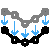
\includegraphics[width=3cm]{Figures/update}
\end{figure*}

Inputs:
\begin{itemize}
    \setlength\itemsep{0.05em}
    \item \textbf{Update Curves} (Update): update Rhino curves to new positions. Attach a boolean button here. {\color{gray}Default: false}. {\color{kpink}\textbf{WARNING:} depending on when this component is triggered, it \textit{may} be a destructive process. IE ctrl+Z at your own risk. Use the FreezeNetwork component to provide a safeguard.}
    \item \textbf{Target Network} (Network): the target network to base curve updates.
    \item \textbf{Edge IDs} (GUIDs): the GUIDs of the input curves to update. These can be extracted using the \textbf{GUID} component in Grasshopper. This component works by matching the GUIDs of drawn geometry (in Rhino) with the GUIDs of the network edges.
\end{itemize}

\subsubsection{Freeze Network (Freeze)}\label{Freeze}
Store a hard copy of the current network.

\begin{figure*}[h]
    \centering
    
\includegraphics[width=3cm]{Figures/export}
\end{figure*}

Inputs:
\begin{itemize}
    \setlength\itemsep{0.05em}
    \item \textbf{Freeze} (Freeze): freeze the network. Attach a boolean button here.
    \item \textbf{Network} (Network): network to freeze
    \item \textbf{Loads} (P): load vectors to freeze
    \item \textbf{Save Directory} (Dir): folder to save data. Must be written with double backslashes.
    \item \textbf{File Name} (Name): name of file to save. Must end in .json.{\color{gray} Default: network.json}
    \item \textbf{Save Offset} (Offset): offset of geometry (curves and points) that is frozen. The default offset is 1.5 times the overall bounding box width in the positive X direction.
\end{itemize}

Outputs:
\begin{itemize}
    \setlength\itemsep{0.05em}
    \item \textbf{Edges} (E): frozen edges
    \item \textbf{Anchors} (A): frozen anchors
    \item \textbf{Force Densities} (q): frozen force densities
    \item \textbf{Network} (Network): frozen network
\end{itemize}

The output reflects the input network at the last time the \textbf{Freeze} button was triggered. Input values can be deleted and the component will retain outputs. In worst-case scenarios, bake the geometry or load the resulting file to restart.

\subsubsection{Load Network (Load)}\label{Load}
Load a saved network .json.

\begin{figure*}[h]
    \centering
    
\includegraphics[width=3cm]{Figures/import}
\end{figure*}

Inputs:
\begin{itemize}
    \setlength\itemsep{0.05em}
    \item \textbf{Folder} (Dir): folder containing file. Must be written with double backslashes.
    \item \textbf{File Name} (Name): name of file to load. Must end in .json
\end{itemize}

Outputs:
\begin{itemize}
    \setlength\itemsep{0.05em}
    \item \textbf{Curves} (Curves): curves that define network
    \item \textbf{Anchors} (Anchors): points that define anchors
    \item \textbf{Force Densities} (q): force density values
    \item \textbf{Loads} (P): vectors that define loads applied to saved network
\end{itemize}

Outputs can directly be connected to a new \textbf{Create Network} component.

\subsubsection{Baker (Baker)} \label{Baker}
Bake the geometry of a network, with edges optionally coloured with respect to a given network property. Use this for exporting final geometries for editing/visualization.

\begin{figure*}[h]
    \centering
    \includegraphics*[width=3cm]{Figures/baker}
\end{figure*}

Inputs:
\begin{itemize}
    \setlength\itemsep{0.05em}
    \item \textbf{Network} (Network): Network to bake.
    \item \textbf{BakeLayer} (Layer): Layer to bake geometry. {\color{gray} Default: "Layer 05"}
    \item For parameters below, see \nameref{Visualize}:
    \subitem Cmin
    \subitem Cmed
    \subitem Cmax
    \subitem Property
    \item \textbf{Bake} (Bake): Bake the geometry with above parameters. {\color{gray} Default: false}
    \item \textbf{BakeOffset} (Offset): Additional offset of baked geometry from reference network; default is set to 1.5x the overall bounding box width in the negative X direction. {\color{gray} Default: [0,0,0]}
\end{itemize}

Outputs:
\begin{itemize}
    \setlength\itemsep{0.05em}
    \item \textbf{Curves} (Curves): Curves of network (\textit{not offset})
    \item \textbf{Anchors} (Anchors): Anchors of network (\textit{not offset})
\end{itemize}

\subsection{Optimization} \label{Optimization}
These components form the core of FDMremote, and requires installation of FDMremote.jl. 

\subsubsection{Remote Start (FDMstart)} \label{FDMstart}
Initializes the connection to the Julia server and generates a WebSocket object.

\begin{figure*}[h]
    \centering
    
\includegraphics[width=3cm]{Figures/start.png}
\end{figure*}

Inputs:
\begin{itemize}
    \setlength\itemsep{0.05em}
    \item \textbf{Reset} (Rst): Reset the connection to the server. In most cases, this input should not be necessary. Connect a Boolean button. {\color{gray} Default: false}
    \item \textbf{Host} (Host): Host address of server. {\color{gray} Default: 127.0.0.1}
    \item \textbf{Port} (Port): Port address of server. {\color{gray} Default: 2000}
\end{itemize}

Outputs:
\begin{itemize}
    \setlength\itemsep{0.05em}
    \item \textbf{WebSocket object} (WSC): WebSocket object that communicates with Julia server 
\end{itemize}

It is recommended to start the Julia server by running \texttt{FDMsolve!()} before using this component.
\subsubsection{Remote Send (FDMsend)} \label{FDMsend}
Send network information to the Julia server.

\begin{figure*}[h]
    \centering
    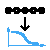
\includegraphics[width=3cm]{Figures/send}
\end{figure*}

Inputs:
\begin{itemize}
    \setlength\itemsep{0.05em}
    \item \textbf{WebSocket object} (WSC): WebSocket object; attach the output of \textbf{FDMstart}
    \item \textbf{Network} (Network): Network to analyze
    \item \textbf{Optimization Parameters} (Params): Parameters for analysis/optimization. {\color{gray} Default: null parameter for a single solve}
    \item \textbf{Load} (P): Applied loads to analyze. {\color{gray} Default: [0,0,0]}
    \item \textbf{Close} (Close): Send a `CLOSE' message to sever connection. {\color{gray} Default: false}  
\end{itemize}

Outputs:
\begin{itemize}
    \setlength\itemsep{0.05em}
    \item \textbf{Network} (Network): a copy of the input network
    \item \textbf{Message} (Msg): A copy of the raw message sent to server
\end{itemize}

\subsubsection{Remote Listen (FDMlisten)} \label{FDMlisten}
Receive and parse messages sent back by server.

\begin{figure*}[h]
    \centering
    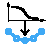
\includegraphics[width=3cm]{Figures/listen}
\end{figure*}

Inputs:
\begin{itemize}
    \setlength\itemsep{0.05em}
    \item \textbf{WebSocket object} (WSC): WebSocket object; attach the output of \textbf{FDMstart}
    \item \textbf{Auto Update} (Upd): Automatically update output values for each new message. {\color{gray} Default: true}
    \item \textbf{Network} (Network): Copy of initial network sent to server. Connect to output of \textbf{FDMsend}
\end{itemize}

Outputs:
\begin{itemize}
    \setlength\itemsep{0.05em}
    \item \textbf{Data} (Data): Raw message received from server
    \item \textbf{Network Status} (Sts): Status of current client-server connection
    \item \textbf{Optimization Finished} (Finished): Status of optimization/solving routine
    \item \textbf{Force densities} (q): Solved force density values
    \item \textbf{Loss} (f(q)): Current objective function value (for optimization)
    \item \textbf{Iteration} (Iter): Current iteration of optimization routine
    \item \textbf{Loss Trace} (f(q(t))): History of objective function value to date
    \item \textbf{Solve Network} (Network): Solved network from optimization
\end{itemize}

\subsubsection{Optimization Parameters (Params)}
Parameters for optimization.

\begin{figure*}[h]
    \centering
    
\includegraphics[width=3cm]{Figures/parameters}
\end{figure*}

Inputs:
\begin{itemize}
    \setlength\itemsep{0.05em}
    \item \textbf{Objective Functions} (Obj): One or more objective functions. {\color{gray} Default: Null Objective}
    \item \textbf{Lower Bound} (LB): Lower bound of q values for optimization. Either a single value or list of values. {\color{gray} Default: 0.1}
    \item  \textbf{Upper Bound} (UB): Upper bound of q values for optimization. Either a single value or list of values. {\color{gray} Default: 100}
    \item \textbf{Absolute Tolerance} (AbsTol): Absolute stopping tolerance. {\color{gray} Default: 1e-3}
    \item \textbf{Relative Tolerance} (RelTol): Relative stopping tolerance (currently not in use).
    \item \textbf{Maximum Iterations} (MaxIter): Maximum iterations during optimization. {\color{gray} Default: 400}
    \item \textbf{Update Frequency} (Frequency): Frequency intermediate messages sent back to client. {\color{gray} Default: 20}
    \item \textbf{Show Iterations} (ShowIter): Send back intermediate messages (primarily for visualization). {\color{gray} Default: true}
\end{itemize}

Outputs:
\begin{itemize}
    \setlength\itemsep{0.05em}
    \item \textbf{Optimization Parameters} (Params): consolidated parameters. Connect to \textbf{FDMsend} 
\end{itemize}

\subsection{Objective Functions} \label{Objectives}
A suite of composable objective functions for optimization. The decision variables are (currently) all edge force densities. All objective functions have a numeric weight that can be adjusted to control relative importance. These weights are \textit{always} relative.

\subsubsection{Target (OBJTarget)} label{OBJTarget}
Match the target shape. Equivalent to minimizing the distance a node travels from its drawn position to the equilibrium position.

$$
OBJ = \lVert \vec{XYZ}_0 - \vec{XYZ}_f \rVert
$$

\begin{figure*}[h]
    \centering
    
\includegraphics[width=3cm]{Figures/Target}
\end{figure*}

Inputs:
\begin{itemize}
    \setlength\itemsep{0.05em}
    \item \textbf{Weight} (W): Objective weight. {\color{gray} Default: 1.0}
\end{itemize}

Outputs:
\begin{itemize}
    \setlength\itemsep{0.05em}
    \item \textbf{Objective} (OBJ): Objective function
\end{itemize}

\subsubsection{StructuralPerformance (OBJFL)} \label{OBJFL}
Proxy for structural performance.

$$
OBJ = \sum_1^{N_e} |F_i|L_i
$$

\begin{figure*}[h]
    \centering
    
\includegraphics[width=3cm]{Figures/performance}
\end{figure*}

Inputs:
\begin{itemize}
    \setlength\itemsep{0.05em}
    \item \textbf{Weight} (W): Objective weight. {\color{gray} Default: 1.0}
\end{itemize}

Outputs:
\begin{itemize}
    \setlength\itemsep{0.05em}
    \item \textbf{Objective} (OBJ): Objective function
\end{itemize}

\subsubsection{ForceVariation (OBJForce)} \label{OBJForce}
Minimize the difference between the largest and smallest forces.

$$
OBJ = \max(F) - \min(F)
$$

\begin{figure*}[h]
    \centering
    
\includegraphics[width=3cm]{Figures/Force var}
\end{figure*}

Inputs:
\begin{itemize}
    \setlength\itemsep{0.05em}
    \item \textbf{Weight} (W): Objective weight. {\color{gray} Default: 1.0}
\end{itemize}

Outputs:
\begin{itemize}
    \setlength\itemsep{0.05em}
    \item \textbf{Objective} (OBJ): Objective function
\end{itemize}

\subsubsection{LengthVariation (OBJLength)} \label{OBJLength}
Minimize the difference between the largest and smallest stressed lengths.

$$
OBJ = \max(L) - \min(L)
$$

\begin{figure*}[h]
    \centering
    
\includegraphics[width=3cm]{Figures/length var}
\end{figure*}

Inputs:
\begin{itemize}
    \setlength\itemsep{0.05em}
    \item \textbf{Weight} (W): Objective weight. {\color{gray} Default: 1.0}
\end{itemize}

Outputs:
\begin{itemize}
    \setlength\itemsep{0.05em}
    \item \textbf{Objective} (OBJ): Objective function
\end{itemize}

\subsubsection{MinimumForce (OBJMinForce)} \label{OBJMinForce}
Penalize all internal forces less than a given value, proportional to the distance away from threshold.

\begin{align*}
    \vec{t} &= \left[v - F_i\right] \; \forall \; i\\
    OBJ &= \sum t_i + |t_i|
\end{align*}

\begin{figure*}[h]
    \centering
    \includegraphics*[width = 3cm]{Figures/minforce}
\end{figure*}

Inputs:
\begin{itemize}
    \setlength\itemsep{0.05em}
    \item \textbf{Weight} (W): Objective weight. {\color{gray} Default: 1.0}
    \item \textbf{Minimum Force} (Force): Threshold force. {\color{gray} Default: 1.0}
\end{itemize}

Outputs:
\begin{itemize}
    \setlength\itemsep{0.05em}
    \item \textbf{Objective} (OBJ): Objective function
\end{itemize}

\subsubsection{MaximumForce (OBJMaxForce)} \label{OBJMaxForce}
Penalize all internal forces less than a given value, proportional to the distance away from threshold.

\begin{align*}
    \vec{t} &= \left[F_i - v\right] \; \forall \; i\\
    OBJ &= \sum t_i + |t_i|
\end{align*}

\begin{figure*}[h]
    \centering
    \includegraphics*[width = 3cm]{Figures/maxforce}
\end{figure*}

Inputs:
\begin{itemize}
    \setlength\itemsep{0.05em}
    \item \textbf{Weight} (W): Objective weight. {\color{gray} Default: 1.0}
    \item \textbf{Maximum Force} (Force): Threshold force. {\color{gray} Default: 10000.0}
\end{itemize}

Outputs:
\begin{itemize}
    \setlength\itemsep{0.05em}
    \item \textbf{Objective} (OBJ): Objective function
\end{itemize}

\subsubsection{MinimumLength (OBJMinLength)} \label{OBJMinLength}
Penalize all stressed lengths less than a given value, proportional to the distance away from threshold.

\begin{align*}
    \vec{t} &= \left[v - F_i\right] \; \forall \; i\\
    OBJ &= \sum t_i + |t_i|
\end{align*}

\begin{figure*}[h]
    \centering
    \includegraphics*[width = 3cm]{Figures/minlength}
\end{figure*}

Inputs:
\begin{itemize}
    \setlength\itemsep{0.05em}
    \item \textbf{Weight} (W): Objective weight. {\color{gray} Default: 1.0}
    \item \textbf{Minimum Length} (Length): Threshold length. {\color{gray} Default: 1.0}
\end{itemize}

Outputs:
\begin{itemize}
    \setlength\itemsep{0.05em}
    \item \textbf{Objective} (OBJ): Objective function
\end{itemize}

\subsubsection{MaximumLength (OBJMaxLength)} \label{OBJMaxLength}
Penalize all stressed lengths less than a given value, proportional to the distance away from threshold.

\begin{align*}
    \vec{t} &= \left[F_i - v\right] \; \forall \; i\\
    OBJ &= \sum t_i + |t_i|
\end{align*}

\begin{figure*}[h]
    \centering
    \includegraphics*[width = 3cm]{Figures/maxlength}
\end{figure*}

Inputs:
\begin{itemize}
    \setlength\itemsep{0.05em}
    \item \textbf{Weight} (W): Objective weight. {\color{gray} Default: 1.0}
    \item \textbf{Maximum Length} (Length): Threshold length. {\color{gray} Default: 1000}
\end{itemize}

Outputs:
\begin{itemize}
    \setlength\itemsep{0.05em}
    \item \textbf{Objective} (OBJ): Objective function
\end{itemize}

\subsection{Experimental} \label{Experimental}
\subsubsection{Edge Control Surface (CtrlSurfQ)} \label{CtrlSurfQ}
Generates a control NURBs surface that assigns element-wise force density values in a controllable manner. Normalized control sliders are automatically generated.

\begin{figure*}[h]
    \centering
    
\includegraphics[width=3cm]{Figures/SurfQ}
\end{figure*}

Inputs:
\begin{itemize}
    \setlength\itemsep{0.05em}
    \item \textbf{Generate} (Generate): Generate the control surface and sliders. {\color{gray} Default: false}
    \item \textbf{Curve} (Curve): Network edges
    \item \textbf{Ucount} (nU): Control point density in direction 1. {\color{gray} Default = 3}
    \item \textbf{Vcount} (nV): Control point density in direction 2. {\color{gray} Default = 3}
    \item \textbf{Surface Offset} (Offset): Offset of displayed control surface. {\color{gray} Default: [0, 0, -300]}
    \item \textbf{Maximum Value} (Max): Value associated with highest point on control surface. {\color{gray} Default: 100}
    \item \textbf{Minimum Value} (Min): Value associated with highest point on control surface. {\color{gray} Default: 0.1}
    \item \textbf{Control Value} (Value): Z-heights of surface control points. {\color{kpink} \textbf{NOTE:} these will be auto-generated by \textbf{Generate}}
    \item \textbf{Show Surface} (Show): Show the control surface. {\color{gray} Default: true}
    \item \textbf{Text Scale} (TextScale): Scale of text tags on control points. {\color{gray} Default: 20}
\end{itemize}

Outputs:
\begin{itemize}
    \setlength\itemsep{0.05em}
    \item \textbf{Surface} (Surface): The control surface
    \item \textbf{Values} (Vals): The values of the control surface in order of network edges. Input into the \textbf{CreateNetwork} component for q values.
\end{itemize}

\subsubsection{Point Control Surface (CtrlSurfP)} \label{CtrlSurfP}
Generates a control NURBs surface that assigns free point-wise force magnitudes in a controllable manner. Normalized control sliders are automatically generated.

\begin{figure*}[h]
    \centering
    
\includegraphics[width=3cm]{Figures/SurfP}
\end{figure*}

Inputs:
\begin{itemize}
    \setlength\itemsep{0.05em}
    \item \textbf{Generate} (Generate): Generate the control surface and sliders. {\color{gray} Default: false}
    \item \textbf{Network} (Network): Network to assign forces to
    \item \textbf{Ucount} (nU): Control point density in direction 1. {\color{gray} Default = 3}
    \item \textbf{Vcount} (nV): Control point density in direction 2. {\color{gray} Default = 3}
    \item \textbf{Surface Offset} (Offset): Offset of displayed control surface. {\color{gray} Default: [0, 0, -300]}
    \item \textbf{Maximum Value} (Max): Value associated with highest point on control surface. {\color{gray} Default: 100}
    \item \textbf{Minimum Value} (Min): Value associated with highest point on control surface. {\color{gray} Default: 0.1}
    \item \textbf{Control Value} (Value): Z-heights of surface control points. {\color{kpink} \textbf{NOTE:} these will be auto-generated by \textbf{Generate}}
    \item \textbf{Show Surface} (Show): Show the control surface. {\color{gray} Default: true}
    \item \textbf{Text Scale} (TextScale): Scale of text tags on control points. {\color{gray} Default: 20}
\end{itemize}

Outputs:
\begin{itemize}
    \setlength\itemsep{0.05em}
    \item \textbf{Surface} (Surface): The control surface
    \item \textbf{Values} (Vals): The values of the control surface in order of free network nodes. Use these values to scale vectors to input into analysis.
\end{itemize}

\subsubsection{Make Helper (Make)} \label{Make}
A utility component that aids the materialization of networks.

\begin{figure*}[h]
    \centering
    \includegraphics*[width=3cm]{Figures/Maker}
\end{figure*}

Inputs:
\begin{itemize}
    \setlength\itemsep{0.05em}
    \item \textbf{Show} (Show): Show visualizations. {\color{gray} Default: true}
    \item \textbf{Network} (Network): Network to analyze.
    \item \textbf{Material Stiffness} (E): Young's modulus of edge. {\color{gray} Default: 100}
    \item \textbf{Area} (A): Cross sectional area of edge. {\color{gray} Default: 10}
    \item \textbf{Show Nodes} (Nodes): Show nodes as enlarged points. {\color{gray} Default: false}
    \item \textbf{Node Radius} (Radius): Radius of node points. {\color{gray} Default: 5}
    \item  \textbf{Colour Gradients} (F0, F1, N0, N1): Colour gradients to distinguish between fixed and free nodes.
    \item \textbf{Edge Thickness} (Thickness): Thickness of edges. {\color{gray} Default: 5}
    \item \textbf{Straight Spacing} (Spacing): Spacing between edges in aligned row visualization. {\color{gray} Default: 10}
    \item \textbf{Show Straight} (Straight): Show aligned edges. {\color{gray} Default: true}
    \item \textbf{Show Projection} (Projection): Show 2D projection. {\color{gray} Default: true}
    \item \textbf{Show Pairs} (Pairs): Show edge-edge pairs between network and visualizations. {\color{gray} Default: false}
    \item \textbf{PairColour} (Cpair): Colour of edge-edge pair lines. {\color{gray} Default: gray}
    \item \textbf{Text Size} (TextSize): Size of text tags. {\color{gray} Default: 3}
    \item \textbf{Show Text} (Text): Show text tags. {\color{gray} Default: true}
    \item \textbf{Text Colour} (Ctext): Colour of text tags. {\color{gray} Default:} black
    \item \textbf{Straight Offset} (StraightOffset); Offset of aligned edge visualization.
    \item \textbf{Projection Offset} (ProjOffset): Offset of 2D projection visualization.
    \item \textbf{Text Offset} (TextOffset): Offset of text tags in Z direction.
    \item \textbf{Pair Indexer} (Indexer): extracts element-wise assembly information given an integer index.
\end{itemize}